\documentclass[12pt,phd,times]{pkmthesis}
\usepackage{amsmath,epsfig,graphicx,setspace,url,float}
\usepackage{pstricks,colortab,pifont}
\usepackage{lscape,multicol,multirow,longtable,subfigure}
\usepackage{booktabs, tabularx, tabularray}
\usepackage{cite, bm}                           % Due to this hyberref will not work for references (PKM on 07/07/08)
\usepackage[english]{babel}
\usepackage[small,bf]{caption}              % Added on 26/08/08
%\usepackage{slashbox} 
\usepackage{csquotes}  
\usepackage{threeparttable}
%\usepackage{adjustbox}                    % Added on 24/10/08 (Senthil)
\setlength{\textfloatsep}{1cm}              % Spacing b/w  float and text (PKM 01/11/08)
%..........................................................................................................................................
\normalem                                   % Added on 01/07/08 to avoid underline in the references
\setlength{\abovecaptionskip}{8pt}          % Added on 08/07/08
\setlength{\belowcaptionskip}{8pt}          % Added on 08/07/08
%..........................................................................................................................................
\usepackage{hyperref}
\usepackage{extra_functions}
%\input{pagesetup_pkm_twoside.tex}           % Modified on 06/07/08, 10/07/08, 15/07/08
%\input{pagesetup_pkm_singleside.tex}       % For Single Sided Document 
\input{pagesetup_pkm_middleside.tex}       % Middle alignment 
\raggedbottom                               % o6/08/08  (Remove Unnecessary space b/w paragraphs)
%******************************************************************************************************************************************

\begin {document}
\setcounter{page}{1} \pagenumbering{roman}  % 03/07/08
\doublespacing                              % or use \baselineskip 12pt (12, 18 and 24)
%*************************************************** FRONT PAGES**********************************************
%\thispagestyle{empty}
%\pdfbookmark{Title}{Title}
%\begin{center}
\fontsize{15.8pt}{19pt}\selectfont
{\bfseries Open-Set AI-Generated Text Detection and Generator Rejection: An Extension of the MAGE In-the-Wild AI Text Detection Framework}
\vspace*{0.25in}
\begin{center}
\large{A} \\
\vspace{0.1in}
\large{\textit{report submitted in fulfillment of Colloqium based on Summer Internship}} \\
\vspace{0.1in}
\large{in} \\
\vspace{0.1in}
\large{Information Technology} \\
\vspace{0.15in}
\large{By} \\
\vspace{0.15in}
{\bfseries\large{B John Wesley : 2022IMT-033}} \\
\vspace{0.2in}
\large{Under the Supervision of} \\
\vspace{0.15in}
{\bfseries\large{Dr. Saswata Roy}} \\
\vspace{0.2in}
\large{Department of Information Technology}
\end{center}
\end{center}
\begin{figure}[!h]
\centerline{\includegraphics*[width = 3cm]{FrontPages/ABV_IIITM_logo.eps}}
\end{figure}
\centerline {\large{ABV-INDIAN INSTITUTE OF INFORMATION TECHNOLOGY}}\\
\centerline{\large{AND MANAGEMENT GWALIOR}} \vspace*{0.05in} 
\centerline{\large{GWALIOR, MADHYA PRADESH, INDIA}}
\vspace*{0.05in}
\centerline{\large{AUGUST, 2026}}

%\thispagestyle{empty}
%\clearpage

\thispagestyle{empty}
\pdfbookmark{Title}{Title}
\begin{center}
\fontsize{15.8pt}{19pt}\selectfont
{\bfseries Open-Set AI-Generated Text Detection and Generator Rejection: An Extension of the MAGE In-the-Wild AI Text Detection Framework}
\vspace*{0.25in}
\begin{center}
\large{A} \\
\vspace{0.1in}
\large{\textit{report submitted in fulfillment of Colloqium based on Summer Internship}} \\
\vspace{0.1in}
\large{in} \\
\vspace{0.1in}
\large{Information Technology} \\
\vspace{0.15in}
\large{By} \\
\vspace{0.15in}
{\bfseries\large{B John Wesley : 2022IMT-033}} \\
\vspace{0.2in}
\large{Under the Supervision of} \\
\vspace{0.15in}
{\bfseries\large{Dr. Saswata Roy}} \\
\vspace{0.2in}
\large{Department of Information Technology}
\end{center}
\end{center}
\begin{figure}[!h]
\centerline{\includegraphics*[width = 3cm]{FrontPages/ABV_IIITM_logo.eps}}
\end{figure}
\centerline {\large{ABV-INDIAN INSTITUTE OF INFORMATION TECHNOLOGY}}\\
\centerline{\large{AND MANAGEMENT GWALIOR}} \vspace*{0.05in} 
\centerline{\large{GWALIOR, MADHYA PRADESH, INDIA}}
\vspace*{0.05in}
\centerline{\large{AUGUST, 2026}}

\thispagestyle{empty}

\clearpage
\thispagestyle{empty}
\pdfbookmark{Declaration}{Declaration}
\begin{center}
{\Large \bf DECLARATION}
\end{center}
\vspace{0.8cm}
\noindent I hereby certify that the work, which is being presented in the report/thesis, entitled {\bf Open-Set AI-Generated Text Detection and Generator Rejection: An Extension of the MAGE In-the-Wild AI Text Detection Framework}, in fulfillment of the requirement for the award of the degree of Master's of Technology and submitted to the institution is an authentic record of my/our own work carried out during the period May-2026 to August-2026 under the supervision of Dr. Saswata Roy. I also cited the reference about the text(s)/figure(s)/table(s) from where they have been taken.

\vspace{2.5cm}

\noindent Dated: \hfill {\bf Signature of the candidate}

\vspace{2cm}

\noindent This is to certify that the above statement made by the candidates is correct to the best of my knowledge.

\vspace{2.5cm}

\noindent Dated: \hfill {\bf Signature of supervisor}


\clearpage
\thispagestyle{empty}
\pdfbookmark{Acknowledgement}{Acknowledgement}
\begin{center}
{\LARGE \bf Acknowledgements}
\end{center}
\noindent I am highly indebted to Dr. Saswata Roy, for his esteemed mentorship, and for allowing me to freely explore and experiment with various ideas in the course of making this project a reality. The leeway I was given went a long way towards helping cultivate a genuine hunger for knowledge and keeping up the motivation to achieve the best possible outcome. I can genuinely say that this Colloquium made me explore many areas of open-set text detection and generator distribution modeling that are new to me, and kindled an interest to further follow up on some of those areas. Moreover, the successful completion of this project has brought with it great satisfaction and more importantly, confidence in my ability to produce more high-quality non-trivial artificial intelligence systems that can make a difference in the real-world. I would like to sincerely express my gratitude to this prestigious institution for providing me and my colleagues with the opportunity to pursue this Colloquium. It is an honor to be able to work on such an important academic project under the guidance and support I am provided with. I am grateful for the resources and facilities provided by this institution, which have been instrumental in enabling me to conduct my research and complete this project. Moreover, I deeply appreciate the efforts of my professors in mentoring and fairly evaluating our works.

\begin{flushright}
\vspace{0.8cm}
{\itshape B John Wesley} \\
{\bfseries 2022IMT-033}
\end{flushright}

\thispagestyle{empty}

\clearpage
\thispagestyle{empty}
\pdfbookmark{Abstract}{Abstract}
\begin{center}
{\LARGE \bf Abstract}
\end{center}
\noindent As large language models (LLMs) proliferate, the threat of academic plagiarism, misinformation, and automated sybil attacks has magnified the need for robust machine-generated text detectors. While supervised classifiers achieve high accuracy in closed-world setups where train and test distributions are identical, they struggle to generalize "in the wild" under severe domain and generator family shifts. Conventional binary detectors forced to select between known classes will incorrectly assign unseen generator text to familiar distributions.

In this work, we reproduce and evaluate multiple AI text detection paradigms (lexical, rank predictability, curvature zero-shot, and contextual deep learning) based on the Association for Computational Linguistics (ACL 2024) MAGE benchmarking framework. We introduce an **academic research extension**: an explicit open-set generator rejection layer integrated into the attribution pipeline. By extracting 768-dimensional contextual final-layer CLS embeddings using a DistilBERT backbone, we model the distributions of known generator families (GPT and LLaMA) using class centroids and regularized covariance matrices. An out-of-distribution (OOD) distance score is computed using the minimum Mahalanobis distance to known centroids, and a validation-tuned threshold (at the 95th percentile) is established under zero-leakage conditions.

Our baseline open-set evaluation against held-out OPT text yields a modest OOD AUROC of $0.6298$ with an OPT rejection rate of $7.59\%$. We conduct three controlled studies: Experiment 1 demonstrates that CLS pooling significantly outperforms mean pooling ($0.6298$ vs. $0.5251$ AUROC); Experiment 2 shows that Cosine distance collapses due to embedding collinearity compared to Mahalanobis distance ($0.4898$ vs. $0.6298$ AUROC); and Experiment 3 establishes partial cross-generator generalization via leave-one-out testing (yielding $0.7587$ AUROC for GPT unseen, but falling to near-random levels for OPT and LLaMA unseen due to representational overlap between open-source models). The findings confirm the feasibility of covariance-scaled open-set rejection for distinct generator families, while highlighting representation collapse as a primary limitation.

\thispagestyle{empty}
\clearpage
%\mbox{}
%\thispagestyle{empty}
%\newpage
%..........................................................................................................................................
% For the fancy chapters (Don't remove these lines- 03/07/08)
\clearpage
\thispagestyle{empty}
\dominitoc
\dominilof
\dominilot
\fancyhf{} \fancyhead[LE]{\bfseries\small{\leftmark}}
\fancyhead[RO]{\bfseries\small{\rightmark}}
\fancyfoot[CE,CO]{\bfseries\thepage}
%..........................................................................................................................................
%TABLE OF CONTENTS
\renewcommand{\baselinestretch}{1}
\pdfbookmark[0]{Index}{index}
\pdfbookmark[1]{Contents}{toc}
\fancyhead[LE]{\bfseries\small{Contents}}
\fancyhead[RO]{\bfseries\small{Contents}}
\tableofcontents
\clearpage
%.........................................................................................................................................
 %LIST OF FIGURES
\pdfbookmark[1]{List of Figures}{lof}
\addstarredchapter{List of Figures}       % PKM 05/07/08 (For more options  refer minitoc.pdf on page 36)
\fancyhead[LE]{\bfseries\small{List of Figures}}
\fancyhead[RO]{\bfseries\small{List of Figures}}
\listoffigures
\clearpage
%..........................................................................................................................................
% LIST OF TABLES
\pdfbookmark[1]{List of Tables}{lot}
\addstarredchapter{List of Tables}         % or use \mtcaddchapter[List of Tables] [Please Refer minitoc.pdf]
\fancyhead[LE]{\bfseries\small{List of Tables}}
\fancyhead[RO]{\bfseries\small{List of Tables}}
\listoftables
\clearpage
%..........................................................................................................................................
% LIST OF ACRONYMS
% \fancyhead[LE]{\bfseries\small{List of Acronyms}}
% \fancyhead[RO]{\bfseries\small{List of Acronyms}}
% \pdfbookmark[1]{List of Acronyms}{loa}
% \addstarredchapter{List of Acronyms}
% \chapter*{List of Acronyms}



\begin{longtable}{ll}

%A


5G & Fifth Generation \\
6G & Sixth Generation \\
CNN & Convolutional Neural Network\\
CR & Cognitive Radio \\
CRN & Cognitive Radio Network \\
CSS & Cooperative Spectrum Sensing \\
DQN & Deep Q-Network \\
DDQN & Double Deep Q-Network \\
DRL & Deep Reinforcement Learning \\
DRQN & Deep Recurrent Q-Network \\
DFT & Discrete Fourier Transform \\
ML & Machine Learning \\
MSE & Mean Squared Error \\
PU & Primary User \\
QN & Q-Network\\
RAM & Random Access Memory \\ 
SNR & Signal to Noise Ratio \\
SS & Spectrum Sensing \\
SU & Secondary User \\
SVD & Singular Value Decomposition \\




%B


%C


%D

     

%E




%F


%G



%H


%I



%J

%K


%L



%M



%N


%O



%P



%Q



%R



%S



%T


%U


%V


%W




%X

%Y

%Z

\end{longtable}

% \clearpage
%..........................................................................................................................................
% LIST OF SYMBOLS
% \fancyhead[LE]{\bfseries\small{List of Symbols}}
% \fancyhead[RO]{\bfseries\small{List of Symbols}}
% \pdfbookmark[1]{List of Symbols}{los}
% \addstarredchapter{List of Symbols}
% %\include{FrontPages/Symbols}
% \clearpage
%..........................................................................................................................................
\fancyhf{}
\fancyhead[LE]{\bfseries\small{\rightmark}}
\fancyhead[RO]{\bfseries\small{\rightmark}}
\fancyfoot[CE,CO]{\bfseries\thepage}
\setcounter{page}{1} \pagenumbering{arabic}
\renewcommand{\labelenumi}{(\roman{enumi})}   % Added on 09/08/2008
%*******************************************************************************************************************************************************************************************


%************************************************ BEGIN CHAPTERS **********************************************
%\fancychapter{Introduction}
\chapter{Introduction}
\vspace{-1cm}

% \noindent \rule{6.6in}{0.01in}
% \emph{This chapter introduces our project, focusing on the integration of advanced machine learning techniques with web application security. It highlights the significance of accurately detecting and classifying malicious web traffic using both traditional and modern models, and outlines the motivation to enhance cybersecurity through more intelligent and adaptive threat detection. By improving the precision of Web Application Firewalls using feature selection methods and ensemble learning, the project aims to strengthen web defenses and ensure more effective mitigation of evolving cyber threats.}
\section{Introduction}\label{Chapter-1-Introduction}
\noindent The rapid growth of large language models (LLMs) has transformed how text is generated. While these systems increase productivity across many sectors, they also present significant challenges to information security, academic integrity, and digital trust. Automated systems can now generate human-like text at scale, making it easy to create deceptive reviews, fake news, or spam that bypasses traditional security check-points. Detecting machine-generated text has therefore become a critical area of study in modern natural language processing (NLP).

\section{The Generalization Gap and Closed-Set Limits}\label{Chapter-1-Generalization-Gap}
\noindent Traditional AI-generated text detectors are built using supervised machine learning models. While they achieve high accuracy (often exceeding $95\%$) on held-out test data from their training distribution, they suffer from a severe performance drop when tested on unseen topics (domain shift) or text generated by different models (generator shift). Supervised models assume a closed-world setup where every input must belong to the classes seen during training, rendering them fragile under real-world, in-the-wild shifts.

When an AI text detector is deployed in the wild, it will inevitably encounter text generated by previously unseen LLM architectures. A closed-set generator attributor (e.g. classifying text as GPT vs. LLaMA) will be forced to select one of the known classes, even if the text was generated by a completely unseen model family (e.g., OPT). An explicit open-set generator rejection layer addresses this by introducing an \texttt{UNKNOWN} class. By modeling the boundaries of known generator distributions, the system can reject anomalous, out-of-distribution text rather than making incorrect attributions.

\section{Motivation}\label{Chapter-1-Motivation}
\noindent Our motivation originates from the need to improve the reliability and generalizability of machine-generated text detectors in real-world scenarios:
\begin{enumerate} 
\item \textbf{Generalization Gap in AI Text Detection:} Most supervised AI detectors perform exceptionally well in "closed-lab" environments where training and test distributions match, but fail under distribution shifts.
\item \textbf{Closed-Set Attributor Limitations:} Existing supervised attribution systems operate under a closed-world assumption, forcing every machine-generated text into a known class (e.g., classifying a text as GPT or LLaMA even if it was generated by OPT).
\item \textbf{Need for Rejection Capability:} A robust detector must have the ability to flag text generated by a previously unseen LLM as \texttt{UNKNOWN} rather than making an incorrect assignment.
\end{enumerate}

\section{Research Objectives}\label{Chapter-1-Objectives}
\noindent The objectives of this project are:
\begin{itemize}
    \item To reproduce a manageable, multi-domain text detection benchmark based on the ACL 2024 MAGE paper.
    \item To implement multiple detection paradigms (lexical, rank-based, zero-shot, and contextual supervised).
    \item To build an explicit open-set generator rejection layer that models known generator embedding distributions.
    \item To evaluate the OOD rejection performance under representation (pooling), distance metric, and cross-generator generalization studies.
\end{itemize}\label{chap:intro}


% \chapter{Literature Review}
% \vspace{-1cm}
% \noindent \rule{6.6in}{0.01in}
% \emph{This chapter reviews existing research on Web Application Firewalls (WAFs) and machine learning-based threat detection. It summarizes traditional rule-based approaches and explores the use of models like KNN, SVM, and Random Forest for identifying malicious traffic. Key research gaps—such as limited adaptability, poor performance on high-dimensional data, and lack of real-time responsiveness—are also highlighted, forming the basis for our proposed solution.}
% \section{Introduction to AI-Generated Text Forensics}
\noindent The rapid evolution of generative artificial intelligence has led to a significant challenge in digital forensics: distinguishing human-written text from machine-generated content. As Large Language Models (LLMs) grow in size and complexity, they generate text that exhibits high semantic coherence, correct grammar, and contextual relevance. While this facilitates automation in content creation and programming, it introduces substantial risks in academic integrity, information security, and public trust. 

Text forensics has emerged as a crucial field to mitigate these risks. Current methodologies can be categorized into three primary tasks:
\begin{enumerate}
    \item \textbf{Binary Detection:} Distinguishing between human-written and machine-generated text.
    \item \textbf{Closed-Set Attribution:} Classifying machine-generated text into one of several predefined generator models (e.g., attributing a text specifically to GPT-4 or LLaMA-2).
    \item \textbf{Open-Set Generator Rejection:} Identifying whether a text was generated by a model that was completely unseen during training, and rejecting it as an unknown source rather than misclassifying it into a known class.
\end{enumerate}

\section{Supervised and Lexical Detection Paradigms}
\subsection{Lexical and N-Gram Methods}
Early text forensics focused on statistical word and character distributions. Lexical classifiers, such as FastText \cite{joulin2016bag}, utilize bag-of-words representations and n-gram frequencies to fit simple linear classifiers. While these models are highly efficient and scale to massive datasets with minimal computational cost, they suffer from key limitations:
\begin{itemize}
    \item \textbf{Contextual Blindness:} They treat text as unordered bags of tokens, ignoring syntax, word ordering, and semantic coherence.
    \item \textbf{Vulnerability to Synonyms:} Simple lexical substitutions (e.g., using synonyms) can easily bypass n-gram detectors.
\end{itemize}

\subsection{Fine-Tuned Transformer-Based Classifiers}
To capture context, researchers fine-tune pre-trained bidirectional transformer encoders (such as BERT \cite{devlin2018bert} or DistilBERT \cite{sanh2019distilbert}) on balanced corpora of human and machine texts. In these models, the representation of the special classification token (\texttt{[CLS]}) in the final layer aggregates the global context of the entire sequence through self-attention.
Supervised transformer models achieve state-of-the-art accuracy on closed-set benchmarks. However, they are highly susceptible to out-of-distribution (OOD) shifts:
\begin{itemize}
    \item \textbf{Domain Shifts:} If a model is trained on news summaries and evaluated on creative writing, its accuracy drops significantly.
    \item \textbf{Generator Shifts:} When exposed to text generated by a model family absent from the training set, supervised classifiers fail to generalize, leading to high false attribution rates.
\end{itemize}

\section{Zero-Shot and Predictability-Based Detectors}
\subsection{Token Probability Predictability}
Zero-shot methods evaluate text without training classifiers on labeled data, relying instead on the internal token probability distributions of a reference language model (like GPT-2). GLTR (Giant Language Model Test Room) \cite{gehrmann2019gltr} represents the foundational work in this category. It computes the rank of each token under the reference model's prediction distribution. Because language models select highly predictable words (top ranks) to maintain fluency, machine-generated text exhibits lower rank entropy compared to human writing, which contains more unpredictable word choices (tail ranks).

\subsection{Curvature-Based Perturbation Methods}
DetectGPT \cite{mitchell2023detectgpt} improves upon probability ranks by evaluating the local curvature of the reference model's log-likelihood space. It perturbs the candidate text by replacing random words with synonyms using a mask-filling model (e.g., DistilRoBERTa) and measures the resulting drop in log-likelihood under the reference LLM. If the original text lies in a local peak of the model's likelihood space, the perturbed texts will show a sharp decrease in likelihood, signaling machine generation. While mathematically robust and require no training, perturbation methods are highly computationally expensive, requiring hundreds of model evaluations per text.

\section{Open-Set Out-of-Distribution (OOD) Rejection}
\subsection{The Open-Set Challenge in Attribution}
Closed-set classifiers operate under the assumption that all evaluation samples belong to the classes present in the training set. In practical scenarios, however, new generator models are continually released. When a closed-set classifier encounters text from an unseen model (e.g., OPT), it is forced to classify it as one of the known models (e.g., LLaMA), causing severe attribution errors.

\subsection{Distance-Based OOD Detection}
To handle open-set attribution, researchers map text representations into high-dimensional embedding spaces (like DistilBERT's 768-D space) and model the distributions of the known classes. The out-of-distribution score is computed based on the distance from the input embedding to the nearest known class distribution.
Traditional Euclidean distance fails in high-dimensional spaces because it treats all embedding dimensions as independent and isotropic. Angular Cosine distance measures only the direction of the vectors, ignoring magnitude variations.
Mahalanobis distance \cite{mahalanobis1936generalized} resolves these issues by scaling the distance by the covariance matrix of the known training distributions:
$$D_M(z) = \min_{c} \sqrt{(z - \mu_c)^T \Sigma_c^{-1} (z - \mu_c)}$$
where $\mu_c$ is the class centroid and $\Sigma_c$ is the regularized class covariance. The covariance scaling accounts for multi-dimensional correlations and variances, expanding the space along direction of high class variation.

\enlargethispage{2\baselineskip}
\subsection{Threshold Selection Strategies}
Selecting an OOD threshold $\tau$ requires balancing the rejection of unseen data against the false rejection of known data. The standard strategy, introduced by Hendrycks and Gimpel \cite{hendrycks2016baseline}, selects $\tau$ as the 95th percentile of the minimum Mahalanobis distances on a known validation set. This guarantees that at least 95\% of the known samples are correctly classified, while establishing a strict boundary to reject unseen generator families as \textbf{UNKNOWN}.
\label{chap:L_survey}


\chapter{Dataset Overview and Preparation}
\vspace{-1cm}
\noindent \rule{6.6in}{0.01in}
\emph{This chapter offers an in-depth discussion on the datasets used in the project, detailing the preprocessing, feature engineering and feature extraction techniques applied on them.}
\section{Dataset Description}\label{Chapter-2-Dataset}
\noindent The effectiveness of any machine learning model is highly dependent on the quality and representativeness of the dataset used. In this project, we reproduce and evaluate detection paradigms using the official MAGE benchmark dataset (\texttt{yaful/MAGE}). The original MAGE benchmark evaluates detectors against a wide array of domains and 27 LLM variants. For our computationally manageable reproduction, we subsample the dataset to focus on three distinct writing domains and three major generator families.

\subsection{Selected Domains}
\begin{enumerate}
    \item \textbf{XSum (Extreme Summarization):} Factual, highly formal news article summaries.
    \item \textbf{ELI5 (Explain Like I'm Five):} Explanatory, informal forum Q\&A responses.
    \item \textbf{WritingPrompts:} Narrative, highly descriptive fictional stories.
\end{enumerate}

\subsection{AI Generator Families}
We study three major generator families, representing distinct architectural origins:
\begin{itemize}
    \item \textbf{GPT family:} Proprietary models aligned via instruction tuning (e.g. GPT-3.5-turbo).
    \item \textbf{LLaMA family:} Open-weights transformer architectures (LLaMA-7B/13B).
    \item \textbf{OPT family:} Open Pre-trained Transformer models (OPT-13B/30B).
\end{itemize}

\section{Data Partitions and Leakage Prevention}\label{Chapter-2-Splits}
To evaluate open-set rejection without data leakage, we construct separate training, validation, and test splits for each leave-one-generator-out configuration. The unseen generator is completely filtered out from training, validation, centroid calculation, covariance calculation, and threshold selection:
\begin{itemize}
    \item \textbf{Experiment 3A (OPT Unseen):} GPT and LLaMA are known. OPT is held out.
    \item \textbf{Experiment 3B (LLaMA Unseen):} GPT and OPT are known. LLaMA is held out.
    \item \textbf{Experiment 3C (GPT Unseen):} LLaMA and OPT are known. GPT is held out.
\end{itemize}

\begin{table}[h]
\centering
\begin{tabular}{lccc}
\toprule
\textbf{Split Profile} & \textbf{3A: OPT Unseen} & \textbf{3B: LLaMA Unseen} & \textbf{3C: GPT Unseen} \\
\midrule
\textbf{Known training set} & 10,000 (GPT + LLaMA) & 10,000 (GPT + OPT) & 10,000 (LLaMA + OPT) \\
\textbf{Known validation set} & 1,000 (GPT + LLaMA) & 1,000 (GPT + OPT) & 1,000 (LLaMA + OPT) \\
\textbf{Known test set} & 1,000 (GPT + LLaMA) & 1,000 (GPT + OPT) & 1,000 (LLaMA + OPT) \\
\textbf{Unseen test set} & 8,012 (OPT) & 3,710 (LLaMA) & 8,084 (GPT) \\
\bottomrule
\end{tabular}
\caption{Dataset partitions and sample counts across Experiment 3 splits.}
\label{tab:dataset_splits}
\end{table}

\section{Feature Extraction and Representation}\label{Chapter-2-Features}
We use the \texttt{distilbert-base-uncased} tokenizer to map raw text into token ID sequences. Text is padded or truncated to a maximum length of 512 tokens.

During the forward pass of DistilBERT, the input sequence is processed through 6 transformer layers. The final hidden state of the first token (the \texttt{[CLS]} token) is extracted as the 768-dimensional sequence representation:
$$\mathbf{z} = \text{last\_hidden\_state}[:, 0, :] \in \mathbb{R}^{768}$$
This vector summarizes the entire contextual information of the text and serves as the style embedding for both attribution and open-set rejection.
\label{chap:problem_statement}


\chapter{Experiment and Results}
\vspace{-1cm}
\noindent \rule{6.6in}{0.01in}
\emph{This chapter covers the description of the experimental setup used in the project, along with a detailed account of the outcomes and results achieved.}
\section{Supervised Binary Classification Results}\label{Chapter-3-Supervised}
\noindent We evaluate the supervised binary text classification performance (Human vs. AI) on our test set. We compare a lightweight lexical baseline (FastText) against our fine-tuned DistilBERT transformer classifier:

\begin{table}[h]
\centering
\begin{tabular}{lccccc}
\toprule
\textbf{Model} & \textbf{Accuracy} & \textbf{AUC} & \textbf{Precision} & \textbf{Recall} & \textbf{F1-Score} \\
\midrule
FastText Baseline & 64.6\% & 0.711 & 67.1\% & 57.3\% & 0.618 \\
DistilBERT Classifier & \textbf{78.4\%} & \textbf{0.925} & \textbf{91.9\%} & \textbf{62.2\%} & \textbf{0.742} \\
\bottomrule
\end{tabular}
\caption{Supervised binary classifier performance on test set.}
\label{tab:supervised_results}
\end{table}

\noindent The DistilBERT classifier significantly outperforms the FastText baseline. It achieves an AUC of $0.925$ and maintains a high precision of $91.9\%$, prioritizing the prevention of "false accusations" (labeling human text as AI).

\section{Baseline Detection Paradigms}\label{Chapter-3-Paradigms}
We implement four detection approaches to compare paradigms:
\begin{enumerate}
    \item \textbf{FastText (Lexical):} Matches character and word n-gram frequencies. Fast but lacks context awareness.
    \item \textbf{GLTR (Predictability):} Measures word probability ranks under GPT-2. Exploits the fact that LLMs choose highly predictable words (top ranks), whereas humans write with higher entropy.
    \item \textbf{DetectGPT-lite (Zero-Shot Curvature):} Perturbs the text using DistilRoBERTa-base and measures likelihood differences under GPT-2. Zero-shot but computationally expensive.
    \item \textbf{DistilBERT (Contextual):} Processes text bidirectionally to capture subtle stylistic footprints.

\end{enumerate}

\section{Proposed Open-Set Rejection Layer}\label{Chapter-3-Novelty}
\noindent To identify and reject text generated by unseen models, we build a Stage-2 open-set rejection layer based on known class distributions.

\subsection{Mathematical Formulation}
For each known class $c \in \{0, 1\}$ (representing known generators GPT and LLaMA), we extract training embeddings $\mathbf{x} \in \mathbb{R}^{768}$ and compute the class centroid:
$$\mu_c = \frac{1}{N_c} \sum_{i=1}^{N_c} \mathbf{x}_i^{(c)}$$
We compute the regularized class covariance matrix:
$$\Sigma_c = \text{Cov}(X^{(c)}) + 10^{-4} \cdot I_{768}$$
The out-of-distribution (OOD) score of a test embedding $\mathbf{z}$ is defined as the minimum Mahalanobis distance to known class distributions:
$$D(\mathbf{z}) = \min_{c \in \{0, 1\}} \sqrt{(\mathbf{z} - \mu_c)^T \Sigma_c^{-1} (\mathbf{z} - \mu_c)}$$
The OOD threshold $\tau$ is chosen as the **95th percentile** of the known validation set's minimum Mahalanobis distances.

\begin{figure}[H]
\centering
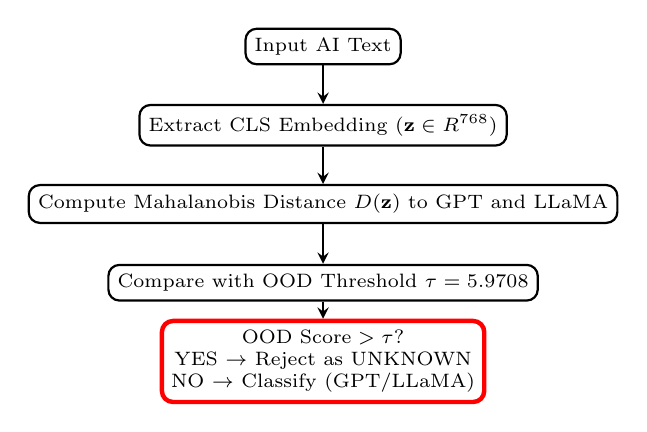
\begin{tikzpicture}[node distance=1.0cm, every node/.style={fill=white, draw=black, rounded corners, thick, align=center, font=\scriptsize}, arrow/.style={thick, ->, >=stealth}]
\node (input) {Input AI Text};
\node (cls) [below of=input] {Extract CLS Embedding ($\mathbf{z} \in \mathbb{R}^{768}$)};
\node (dist) [below of=cls] {Compute Mahalanobis Distance $D(\mathbf{z})$ to GPT and LLaMA};
\node (thresh) [below of=dist] {Compare with OOD Threshold $\tau = 5.9708$};
\node (decision) [below of=thresh, draw=red, ultra thick] {$\text{OOD Score} > \tau$? \\ YES $\to$ Reject as UNKNOWN \\ NO $\to$ Classify (GPT/LLaMA)};

\draw [arrow] (input) -- (cls);
\draw [arrow] (cls) -- (dist);
\draw [arrow] (dist) -- (thresh);
\draw [arrow] (thresh) -- (decision);
\end{tikzpicture}
\caption{Open-set generator rejection pipeline flow.}
\label{fig:pipeline_flow}
\end{figure}

\section{Baseline Open-Set Rejection Results}\label{Chapter-3-Baseline}
In our baseline configuration (unseen: OPT, known: GPT + LLaMA, representation: CLS, distance: Mahalanobis):
\begin{itemize}
    \item \textbf{Selected Threshold ($\tau$):} $63.5972$
    \item \textbf{OPT Unknown Rejection Rate:} $7.59\%$ (608 / 8,012 OPT samples flagged)
    \item \textbf{Known Class False Rejection:} $3.90\%$ (39 / 1,000 known test samples incorrectly flagged)
    \item \textbf{OOD Score AUROC:} $0.6298$
\end{itemize}
The baseline OOD AUROC ($0.6298$) represents modest separation. While it maintains a low false rejection rate, only a small fraction of the unseen OPT family is successfully rejected.

\section{Experiment 1: Representation Pooling Study}\label{Chapter-3-Exp1}
We evaluate the representation extraction method, comparing CLS token pooling against attention-mask-aware mean pooling:
\begin{table}[h]
\centering
\begin{tabular}{lccc}
\toprule
\textbf{Metric} & \textbf{Baseline (CLS Pooling)} & \textbf{Experiment 1 (Mean Pooling)} & \textbf{Delta} \\
\midrule
\textbf{Unseen OPT Rejection} & \textbf{7.59\%} & \textbf{1.61\%} & -5.98\% \\
\textbf{Known False Rejection} & \textbf{3.90\%} & \textbf{4.40\%} & +0.50\% \\
\textbf{Open-Set OOD AUROC} & \textbf{0.6298} & \textbf{0.5251} & -0.1047 \\
\textbf{OOD Threshold} & 63.5972 & 5.8443 & -57.7529 \\
\bottomrule
\end{tabular}
\caption{Experiment 1 representation pooling results.}
\label{tab:exp1_results}
\end{table}

\noindent Mean pooling drops performance to near-random ($0.5251$ AUROC). Since classification fine-tuning concentrates style features into the \texttt{[CLS]} token, averaging across all tokens averages in semantic domain signatures, washing out generator styles.

\section{Experiment 2: Distance Metric Study}\label{Chapter-3-Exp2}
We compare Mahalanobis distance against Cosine distance:
\begin{table}[h]
\centering
\begin{tabular}{lccc}
\toprule
\textbf{Metric} & \textbf{Baseline (Mahalanobis)} & \textbf{Experiment 2 (Cosine)} & \textbf{Delta} \\
\midrule
\textbf{Unseen OPT Rejection} & \textbf{7.59\%} & \textbf{0.85\%} & -6.74\% \\
\textbf{Known False Rejection} & \textbf{3.90\%} & \textbf{3.70\%} & -0.20\% \\
\textbf{Open-Set OOD AUROC} & \textbf{0.6298} & \textbf{0.4898} & -0.1400 \\
\textbf{OOD Threshold} & 63.5972 & 0.0158 & -63.5814 \\
\bottomrule
\end{tabular}
\caption{Experiment 2 distance metric results.}
\label{tab:exp2_results}
\end{table}

\noindent Cosine distance collapses completely (AUROC = $0.4898$, below random). Fine-tuning collapses embeddings into a collinear cone. Without covariance scaling to expand style variations, angular distance cannot separate the distributions.

\section{Experiment 3: Generalization Study}\label{Chapter-3-Exp3}
We evaluate three leave-one-generator-out configurations under strict no-leakage partitions:
\begin{table}[h]
\footnotesize
\centering
\begin{tabular}{lccc}
\toprule
\textbf{Metric} & \textbf{3A: OPT unseen} & \textbf{3B: LLaMA unseen} & \textbf{3C: GPT unseen} \\
\midrule
\textbf{Known Generators} & GPT + LLaMA & GPT + OPT & LLaMA + OPT \\
\textbf{Unseen Generator} & OPT & LLaMA & GPT \\
\textbf{Threshold} & \textbf{5.9708} & \textbf{57.8356} & \textbf{72.8708} \\
\textbf{Unknown Rejection} & \textbf{1.41\%} & \textbf{5.12\%} & \textbf{27.85\%} \\
\textbf{Known False Rejection} & \textbf{4.10\%} & \textbf{6.40\%} & \textbf{5.80\%} \\
\textbf{OOD AUROC} & \textbf{0.5263} & \textbf{0.4919} & \textbf{0.7587} \\
\bottomrule
\end{tabular}
\caption{Experiment 3 cross-generator generalization results.}
\label{tab:exp3_results}
\end{table}

\noindent GPT is highly separable ($0.7587$ AUROC, $27.85\%$ rejection) because its proprietary alignment differs substantially from open models. LLaMA unseen collapses ($0.4919$ AUROC) due to structural overlap with the OPT family in pre-training.

\section{Domain-Wise Performance Analysis}\label{Chapter-3-Domains}
We break down the OOD AUROC performance across writing domains:
\begin{table}[h]
\centering
\begin{tabular}{lccc}
\toprule
\textbf{Unseen Generator} & \textbf{XSum AUROC} & \textbf{ELI5 AUROC} & \textbf{WritingPrompts AUROC} \\
\midrule
OPT (3A) & 0.5307 & 0.5340 & 0.4698 \\
LLaMA (3B) & 0.4555 & 0.3963 & 0.5609 \\
GPT (3C) & \textbf{0.6665} & \textbf{0.8006} & \textbf{0.7836} \\
\bottomrule
\end{tabular}
\caption{Domain-wise OOD score AUROC across leave-one-out configurations.}
\label{tab:domain_auroc}
\end{table}

\noindent Open-set performance varies heavily across writing styles, with creative writing (WritingPrompts) and forum answers (ELI5) showing much stronger OOD separation for GPT than news articles (XSum).
\label{chap:results}


\chapter{Challenges Faced and Conclusion}
\vspace{-1cm}
\noindent \rule{6.6in}{0.01in}
\emph{This chapter of the report is dedicated to the challenges faced and future scope. This section presents a thorough summary of the principal discoveries and understandings attained through the research conducted in the preceding sections.}
\section{Challenges Faced}\label{Chapter-4-Challenges}
\noindent Several key technical challenges were encountered during the design, implementation, and evaluation of the open-set generator rejection pipeline:
\begin{enumerate}
    \item \textbf{Representation Collapse under Fine-Tuning:} Standard cross-entropy fine-tuning of DistilBERT for generator classification optimizes the model to maximize class separability at the linear decision boundary. However, this process collapses the intra-class feature variance, compressing the 768-dimensional representations of the \texttt{[CLS]} token. Consequently, the minimum Mahalanobis distance ranges become narrow and highly overlapping, making it difficult for the threshold to isolate unseen distributions.
    \item \textbf{High Collinearity of Open-Source Model Families:} The open-weights model families (LLaMA and OPT) share substantial similarities in their underlying transformer architectures, tokenizers, and pre-training web corpora. As a result, their contextual representations are close in the embedding space, making them nearly indistinguishable under distance-based open-set rejection boundaries.
    \item \textbf{Domain Style Interference:} Text representations are heavily influenced by the semantic topic and writing style of the domain. This domain-specific signal is much stronger than the subtle stylistic footprint of the generator, causing the detector to struggle under joint domain and generator shifts.
\end{enumerate}

\section{Conclusions}\label{Chapter-4-Conclusions}
\noindent In this work, we reproduced and benchmarked text detection paradigms based on the ACL 2024 MAGE paper and implemented an explicit open-set generator rejection layer. Our controlled experiments verified that:
\begin{itemize}
    \item Sequence classification fine-tuning aligns style gradients directly into the \texttt{[CLS]} token, making CLS pooling significantly outperform mean pooling.
    \item Mahalanobis distance outperforms Cosine distance by scaling the feature space according to class covariance structure, suppressing collinearity noise.
    \item The system generalizes partially, showing high separation capacity for proprietary instruction-aligned models (GPT) but struggling to separate open-weights models (LLaMA and OPT).
\end{itemize}
The findings support the feasibility of covariance-scaled open-set rejection for distinct generator families, while demonstrating the necessity of metric representation learning to mitigate feature collapse.

\section{Future Scopes}\label{Chapter-4-Future}
\noindent To address these limitations, future research will explore the following directions:
\begin{itemize}
    \item \textbf{Contrastive Representation Learning:} Incorporating contrastive loss (e.g., InfoNCE) or triplet loss during fine-tuning. This will explicitly optimize the model to minimize intra-class distance (maximizing tightness of known generator clusters) and maximize inter-class distance (pushing different families apart), preserving variance and improving OOD boundaries.
    \item \textbf{Multi-Task Pre-Training:} Training on auxiliary tasks (such as domain classification or MLM) to prevent feature collapse and retain generalized stylistic features.
    \item \textbf{Generator Scaling:} Evaluating the boundaries across a larger suite of open-weights models (e.g., Mistral, Bloom, Gemma) and model scales.
    \item \textbf{Calibration Analysis:} Testing threshold calibration techniques to improve OOD scoring robustness.
\end{itemize}\label{chap:conclusion and future scopes}

%**************************************************BIBLIOGRAPHY********************************************************
\fancyhead[LE]{\bfseries\small{Bibliography}}
\fancyhead[RO]{\bfseries\small{Bibliography}}
\pdfbookmark[1]{Bibliography}{los}
\addstarredchapter{Bibliography}   % PKM 05/07/08 (For more options refer minitoc.pdf on page 36)
\baselineskip 11pt
\small
\nocite{*}
\bibliographystyle{IEEEtran}
\let\oldclearpage\clearpage
\let\clearpage\relax
\let\cleardoublepage\relax
\bibliography{MyBibliography_database}
\let\clearpage\oldclearpage

%**************************************************PUBLICATIONS****************************************************************************************************************
\end{document}
